\documentclass[UTF8,a4paper,11pt]{article}

\usepackage{ctex} 
\usepackage{fancyhdr}
\usepackage{multicol} 
\usepackage{lastpage} 
\usepackage{geometry} 
\usepackage{hyperref}
\usepackage{titlesec} 
\usepackage{mathrsfs}
\usepackage{graphicx}
\usepackage{epstopdf}
\usepackage{ulem}
\usepackage{caption}
\usepackage{bm}%专门处理数学粗体的bm宏包
\usepackage{amsmath}
\usepackage[subfigure,AllowH]{graphfig} 

\geometry{left=3cm,right=3cm,top=2.5cm,bottom=2.5cm}
\renewcommand{\baselinestretch}{1.5}
\everymath{\displaystyle}


\title{\huge\heiti 学习笔记(5.27-6.3)}
\author{陈书杰}
\date{\today}

\begin{document}
\maketitle
\thispagestyle{empty}
\begin{figure}[htbp]
\centering
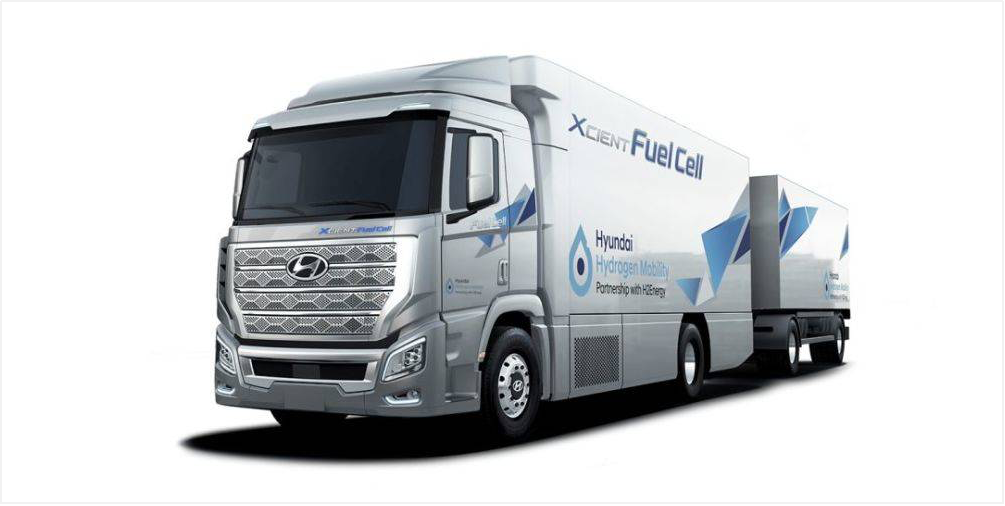
\includegraphics[scale=0.3]{first.jpg}
\end{figure}
\clearpage

\tableofcontents
\setcounter{page}{1}
\pagenumbering{Roman}

\clearpage

\setcounter{page}{1}
\pagenumbering{arabic}
\section{电动汽车概述}
在看这方面的教材的时候,我发现教材中有大量的力学公式的推导。个人认为车辆的动力学方程、传动理论和牵引力计算应该不是重点,因此没有重点看,也不在这边写了。

电动汽车(EV)采用电动机为牵引装置,并应用化学蓄电池组、燃料电池组、超级电容器组或飞轮组为其相应的能源。电动汽车具有胜过传统内燃机车辆(ICEV)的许多优点,例如零排放、高效率、与石油无关以及安静、平稳地运行。以前,从现有的内燃机车辆变换为电动汽车,主要是应用电动机驱动装置和蓄电池组件替代内燃机和燃油箱, 而保留所有其他组件。 但诸如其重型的重量、较低的灵活性以及车辆性能下降等缺陷已导致这类型式电动汽车的逐渐消失。现代电驱动系概念性地示于图1中。该电驱动系由三个主要的子系统组成:电动机驱动、能源和辅助子系统。电动机驱动子系统由车辆控制器、电力电子变换器、电动机、机械传动装置和驱动轮组成;能源子系统包含能源、能量管理单元和能量的燃料供给单元;辅助子系统由功率控制单元、车内气候控制单元和辅助电源组成。


\begin{figure}[htbp]
\centering
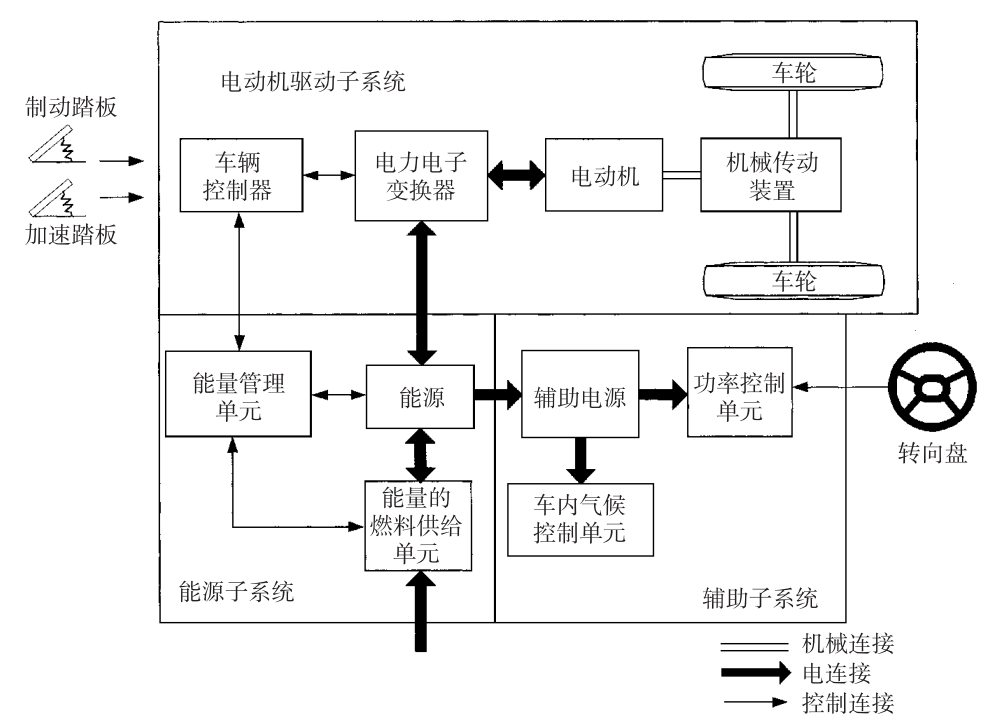
\includegraphics[scale=0.6]{p1.png}
\caption{通用EV结构图}
\end{figure}

车辆的行驶性能通常由其加速时间、最高车速和爬坡能力予以评价。在EV驱动系设计中,固有的电动额定功率和传动装置参数是为满足性能技术要求首要考虑的问题,此处不再赘述。此外,电驱动系统的设计也不是要重点了解的(这似乎是一个单独的学科方向,其内容非常复杂难懂)。

\section{氢氧燃料电池——一种高效率、低排放的动力方案}
\subsection{氢氧燃料电池的基本设计}
近十年来,在车辆中,燃料电池的应用已是人们注意力的焦点所在。与化学蓄电池形成对比,燃料电池产生电能而不储存电能,并且只要维持燃料供给,它将继续运行。相比于配置蓄电池的电动汽车, 配置燃料电池的车辆具有行程较长而无需过长的蓄电池充电时间的优点;相比于内燃机车辆,它具有高能量效率和低得多的排放的优点,因为其燃料中的自由能直接转换为电能,而不经历燃烧过程。

燃料电池是一种原电池,借助于电化学过程,其内部燃料的化学能直接转换为电能。 燃料和氧化剂持续且独立地供给电池的两个电极,并在电极处进行反应。电解液必须用以为离子从一个电极传导至另一极,如图2所示。燃料供给阳极或正极,在该电极处,依靠催化剂,电子从燃料中释放。在两电极间电位差作用下,电子经外电路流向阴极或负极,在阴极处,正离子和氧结合,产生反应物或废气。关于燃料电池的化学动力学分析,此处不赘述。

\begin{figure}[htbp]
\centering
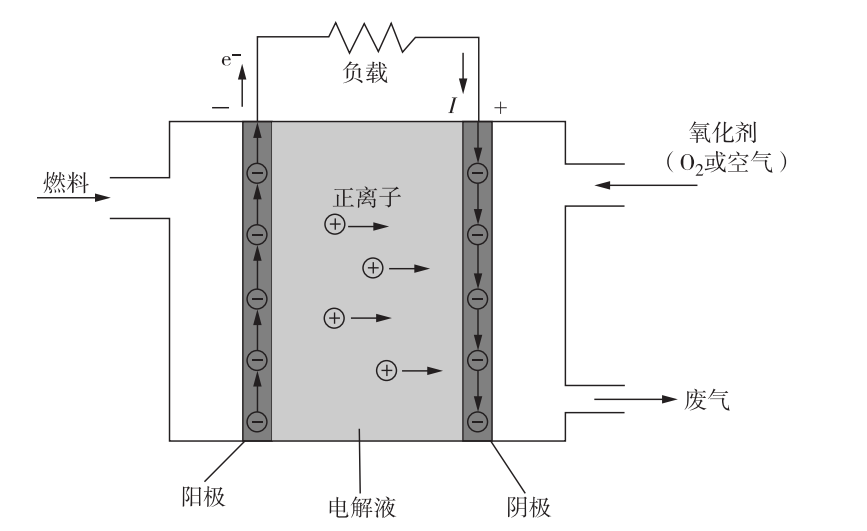
\includegraphics[scale=0.6]{p2.png}
\caption{燃料电池基本运作过程}
\end{figure}

燃料电池的效率曲线与其电压曲线严格相似。氢氧燃料电池的效率-电流曲线如图3所示。 图3表明,随着电流增加,效率下降而功率增加。因此,在低电流下运用燃料电池,即在低功率下可获得高运行效率。然而, 考虑其辅助设备 ( 如空气循环泵、 冷却水循环泵等)所消耗的能量, 由于辅助设备的功率消耗占有较大的百分比, 故很低功率(10\% 的最大功率) 的运行, 将导致较低的运行效率。 

实际上,燃料电池需要辅助设备支持其运行。 辅助设备主要包括空气循环泵、冷却水循环泵、 排气扇、 燃料供应泵和电控设备, 如图4所示。 辅助设备中, 空气循环泵的能量消耗最大, 其消耗功率 (含其驱动电动机) 大约可占燃料电池堆总输出功率的10\%,其他辅助设备消耗的能量比空气循环泵消耗的能量要小得多。

\begin{figure}[htbp]
\centering
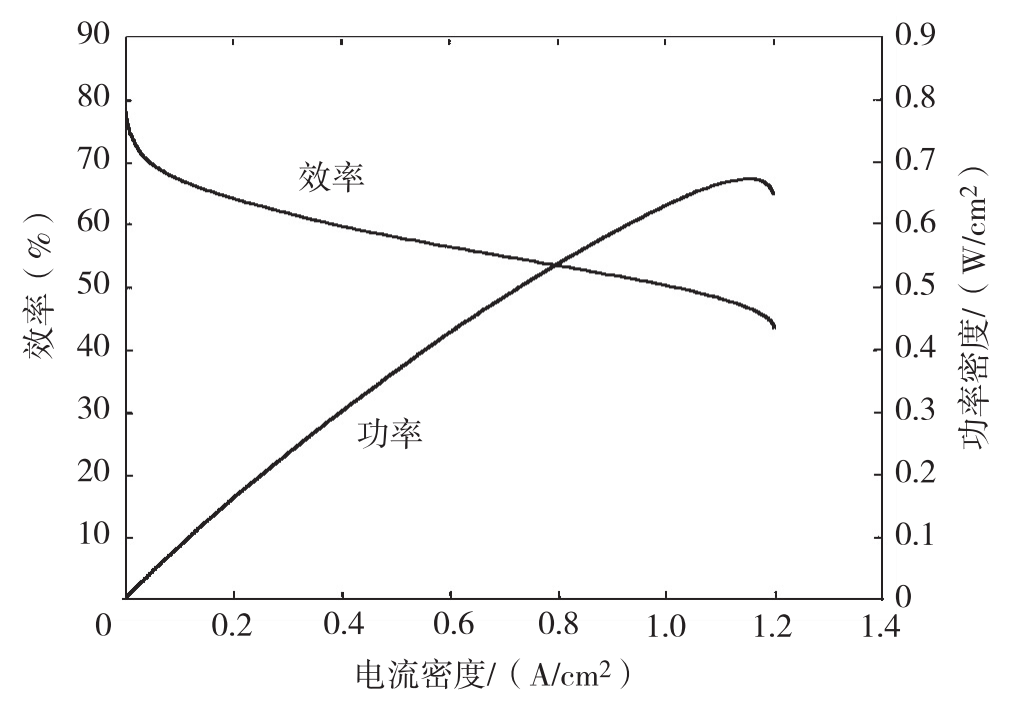
\includegraphics[scale=0.45]{p3.png}
\caption{氢氧燃料电池中的运行效率和功率密度随着电流密度的变化}
\end{figure}

\begin{figure}[htbp]
\centering
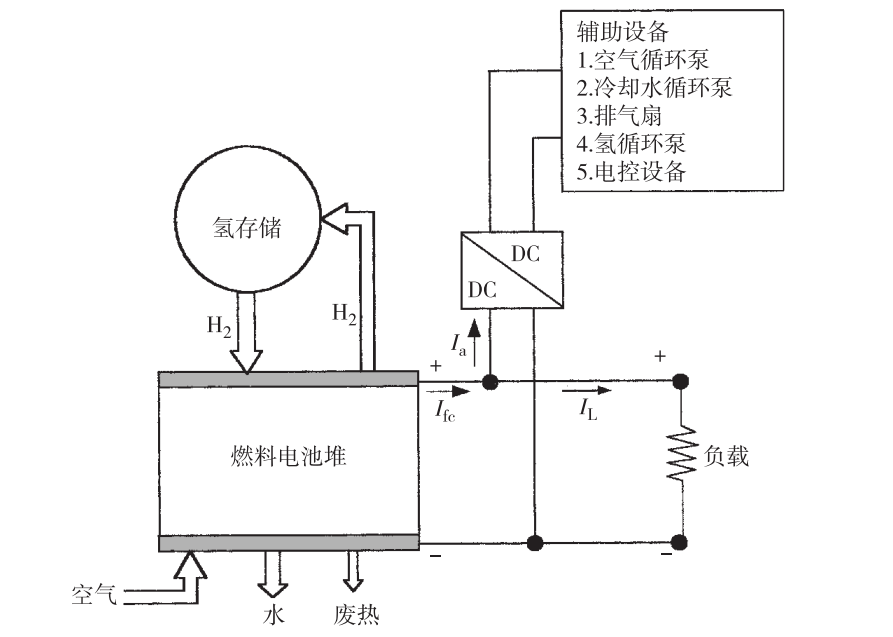
\includegraphics[scale=0.6]{p4.png}
\caption{氢-空气燃料电池系统}
\end{figure}

\subsection{燃料电池的分类}
取决于燃料电池电解质的类型, 可将其分类为六种主要的燃料电池: 质子交换膜 (PEM) 或聚合物交换膜燃料电池 (PEMFC)、 碱性燃料电池 (AFC)、磷酸燃料电池 (PAFC)、 熔融碳酸盐燃料电池 (MCFC)、 固态氧化物燃料电池(SOFC) 和直接甲醇燃料电池 (DMFC)。下面介绍最常用的PEM和AFC。

质子交换膜燃料电池采用固态聚合物膜为电解质。 该聚合物膜为全氟磺酸膜,是酸性的, 因此迁移的离子为氢离子或质子。 质子交换膜燃料电池由纯氢和作为氧化剂的氧或空气一起供给燃料。

聚合物电解质膜被碳基催化剂所覆盖, 催化剂直接与扩散层和电解质两者接触以求达到最大的相互作用面。 催化剂构成电极, 在其之上直接为扩散层。电解质、 催化剂层和气体扩散层的组合被称为膜片—电极组件。质子交换膜燃料电池中的催化剂是关键性的焦点所在。 在早期实践中, 为了燃料电池的特定运行, 需要很可观的铂载量。 在催化剂技术方面现已取得了巨大进展, 使铂载量从$28mg/cm^2$减少到 $0.2mg/cm^2$。 由于燃料电池的低运行温度以及电解质酸性的本质, 故应用的催化剂层需要贵金属。 因氧的催化还原作用比氢的催化氧化作用更为困难, 所以阴极是最关键的电极。


在质子交换膜燃料电池中, 另一关键性问题是水的管理。 为了燃料电池的特定运行, 聚合物膜必须保持湿润。 事实上, 聚合物膜中离子的导电性需要湿度。若聚合物膜过于干燥, 就没有足够的酸离子去承载质子; 若聚合物膜过于湿润(被浸渍), 则扩散层的细孔将被阻断, 从而反应气体不能扩展触及催化剂。

水在质子交换膜燃料电池中的阴极生成。 通过将燃料电池保持在某一温度下,并靠流动足以使水蒸发, 即可令其迁移, 且以水蒸气态移出燃料电池。 然而, 由于误差范围很窄, 故这一方法是困难的。 某些燃料电池堆运行在空气远远过量的状态, 这理应正常地干燥燃料电池, 而同时采用外部增湿器由阳极供水。
 
碱性燃料电池采用含水氢氧化钾 (KOH) 溶剂为电解液, 以传导电极之间的离子。 氢氧化钾是碱性的。 因为电解液为碱性, 故离子传导机理不同于质子交换膜燃料电池。 被碱性电解液迁移的离子是氢氧离子 , 这对燃料电池若干其他方面产生影响。

不同于酸性燃料电池, 水是在氢电极处生成的。 此外, 在阴极处, 氧的还原需要水。 水的管理问题往往按电极防水性和在电解液中保持含水量的需求予以分解。 阴极反应从电解液中消耗水, 而其中阳极反应则排出其水生成物。 过剩的水 (每次反应 2mol) 在燃料电池堆外气化。

碱性燃料电池可以运行在一个宽温度(80~230℃)和压力(2.2~45 个标准大气压)范围内。 高温的碱性燃料电池也可使用高浓度电解液, 该高浓度致使离子迁移机理从水溶剂转换成熔融盐状态。

因由氢氧电解液所提供的快速动力学效应, 故碱性燃料电池可获得很高的效率。 尤其是氧的反应 比酸性燃料电池中氧的还原反应容易得多,因此活性损耗非常低。 碱性燃料电池中的快速动力学效应使银或镍可用以替代铂作为催化剂, 这样碱性燃料电池堆的成本显著下降。

通过电解液完全的循环, 碱性燃料电池动力学特性得到了进一步的改善。 当电解液循环时, 燃料电池被称为 “动态电解液的燃料电池”。 这样一类结构的优点是:由于电解液被用作冷却介质, 因此易于热管理; 更为均匀的电解液的集聚, 解决了阴极周围电解液浓度分布问题; 提供了利用电解液进行水管理的可能性; 如果电解液已被二氧化碳过度污染, 则有替换电解液的可能性; 最终当燃料电池堆关闭, 且其具有可显著延长使用寿命的潜能时, 提供了从燃料电池内移置电解液的可能性。

\begin{figure}[htbp]
\centering
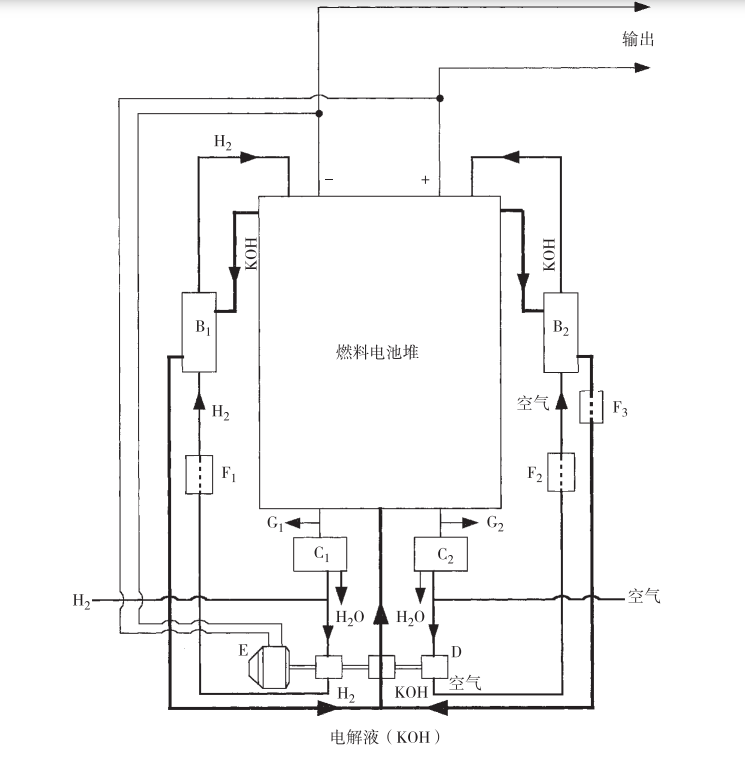
\includegraphics[scale=0.75]{p5.png}
\caption{在碱性燃料电池中循环的电解液和氢与空气的供给}
\end{figure}

但是, 循环电解液的利用, 提出了某些问题, 其中最突出的问题是增加了泄漏的风险: 氢氧化钾是高腐蚀性的, 并具有自然渗漏, 甚至于透过密封的可能性。此外, 循环泵和热交换器的结构, 以及最后的气化器均更为复杂。 另一问题在于,如果电解液被过于激烈地循环或单元电池没有完善地绝缘, 则在两单元电池间将存在内部电解质短路的风险。 循环电解液的碱性燃料电池结构如图5所示。图中,B1、B2是热交换器,C1、C2是冷却器,D是泵,E是电动机,F1、F2、F3是控制器,G1、G2是排气口。

\section{氢能源重卡现状}
\subsection{氢能源重卡的优势}
2020年以来氢燃料电池在乘用车上的使用处处碰壁,存储、续航难题迟迟无法技术攻关。2020年4月,奔驰汽车的母公司就正式宣布停止了乘用车氢燃料电池的研发计划。2021年6月,上海汽车集团发布公告决定终止燃料电池汽车前瞻技术项目的研发。本田、丰田等日本车企,也相继在去年宣布停止氢燃料电池研发。

氢能汽车产业链远比传统汽车产业链更长、复杂度更大。乘用车上的碰壁反而加速了氢能在商用车领域的应用。氢能重卡逐渐成为时代的“宠儿”。根据Nikola的测算,全球重卡市场超过6000亿美元,预计在2030年超过50\%的重卡都将使用氢能。2021年,我国氢能重卡在新能源重卡中销量增速最快,同比增长超33倍;2021年前9月交付客户的氢能重卡有400余台,远超2020年17台的销量。

为什么会造成这样的情况?首先,氢能重卡在加氢站上的投入要远小于乘用车。 重卡主要用于物流配送,其路线相对固定,以高速公路为主。而高速公路布局是节点式的,配套加氢站可以依托于高速网络中的交通枢纽建立,成本大幅降低。例如,我国山西阳泉建设的氢能重卡示范加氢站,一天就可满足固定路线上70辆氢能重卡的加氢需求。 

其次,重卡可大幅缓解氢能成本困境。具体而言,氢能乘用车的使用成本无法和电动轿车、油车的同台竞技,但氢能重卡已经有能力同柴油车和电动车一较高下。在乘用车领域,氢能汽车快速加氢的优势难以发挥。乘用车用户能够忍受电动车的长时间充电,因为这部分时间可以经由上班时间或者夜间进行消纳。但对于货运来说,长途运输要花费几天的时间,电池动辄几小时的充电时间是难以接受的时间成本。

此外,氢能重卡的技术也没有乘用车这么复杂。究其原因,在重卡的车体外部有大量的空间能挂载庞大的储氢系统,不需要像乘用车一样把一套复杂的储氢系统塞进狭小的轿车空间。例如,中国重汽最新研发的黄河氢燃料重卡就在车头后方悬挂储存系统,单次可加氢29.5kg,提供约560km的续航里程。 

\subsection{近期国产氢能源卡车概述}

在搜集国产设备资料的时候,我发现可能是商业机密的原因,大多数设备几乎没有详细的设计图纸和说明,因此此处只能概述。

中国氢能重卡行业尚处于发展初期,产业链环节较少,核心环节在于上游的燃料电池系统与氢内燃机供应,技术壁垒较高。氢能重卡产业链上游为燃料电池系统与氢内燃机供应商,其中燃料电池系统的技术发展更为领先,质子交换膜燃料电池是当前在汽车上装机应用最广的燃料电池,氢内燃机作为新兴崛起的氢能应用技术路线,广受各大车企关注,但整体仍处于研发与探索阶段,尚未实现规模化量产。由此可见,上游动力装置的技术、规模是制约产业发展的重要因素。产业链中游为氢能重卡制造商,整体竞争格局较为分散,头部企业2022年销售市场份额在20\%左右,尚未形成垄断局面,当前氢能重卡在中国重型卡车领域市场渗透率较低,作为国家政策的明确支持方向,市场增长潜力巨大,随着2021年氢内燃机技术被纳入工业绿色发展规划,氢能重卡技术路线将呈现多元化发展,竞争格局有望进一步分散。产业链下游为交通物流运营商,交通物流业作为支撑国民经济的基础性、战略性、先导性产业,市场规模较大并呈稳定增长态势,将通过推进精益化运营、科技创新等实现提质增效,对新能源商用车的需求也将持续扩大。

对于燃料电池系统供应商,主要参与方有北京亿华通科技股份有限公司、潍柴动力股份有限公司、山西美锦能源股份有限公司等。例如亿华通主流的氢燃料电堆,零部件国产化率高达100\%。最高质量功率密度突破800W/kg,实现-35℃低温启动、-40℃低温储存。可广泛适用于公交、物流、城际客车、重卡、环卫车、渣土车等多种车型,如图6。

\begin{figure}[htbp]
\centering
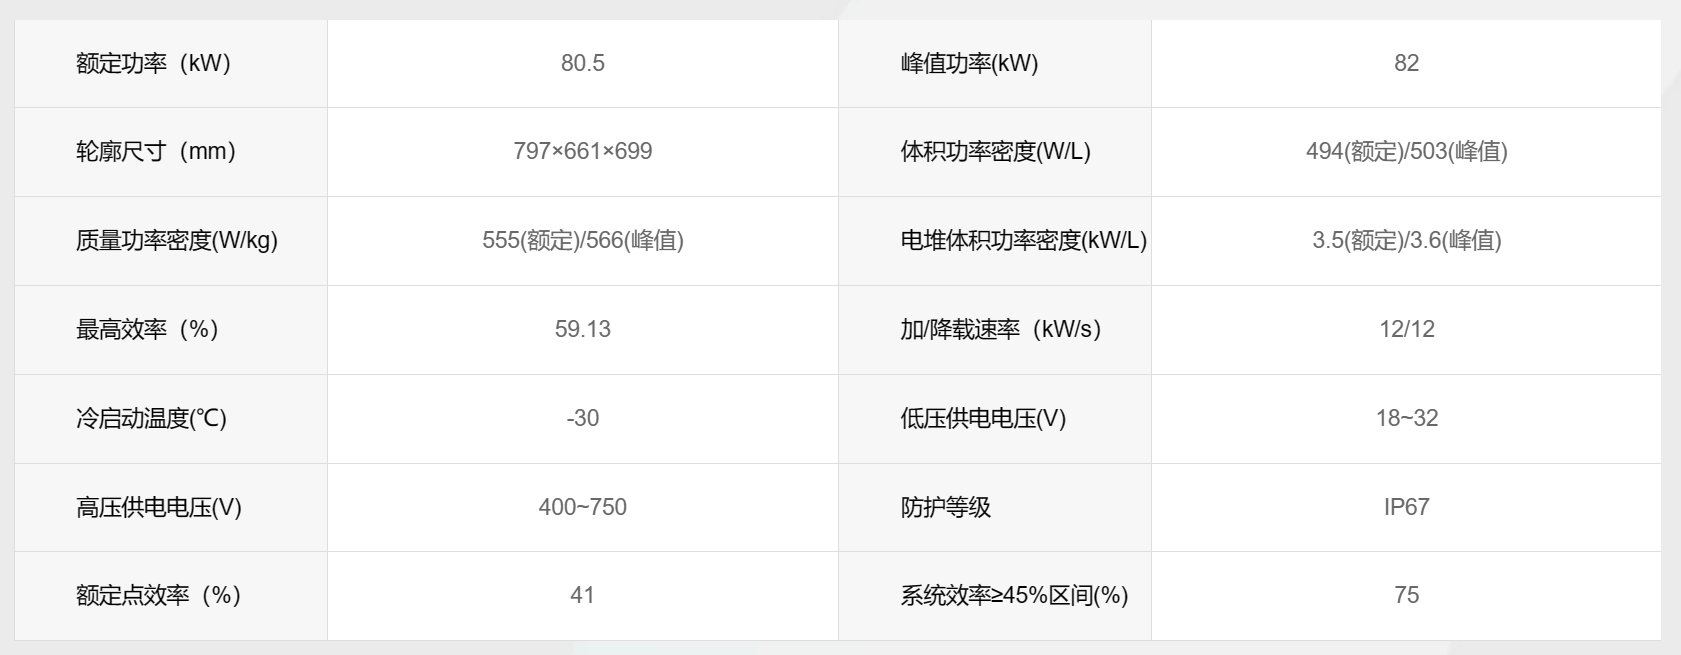
\includegraphics[scale=0.3]{p6.png}
\caption{亿华通主流的氢燃料电堆参数}
\end{figure}

对于氢能重卡生产商,主要参与方有一汽解放集团股份有限公司、东风汽车股份有限公司、三一集团有限公司等。例如三一重工推出的420氢燃料自卸车(如图7),在整备质量18吨的情况下,最高车速可达85km/h,加氢在20分钟以内可以完成,且有良好的操纵性能。

\begin{figure}[htbp]
\centering
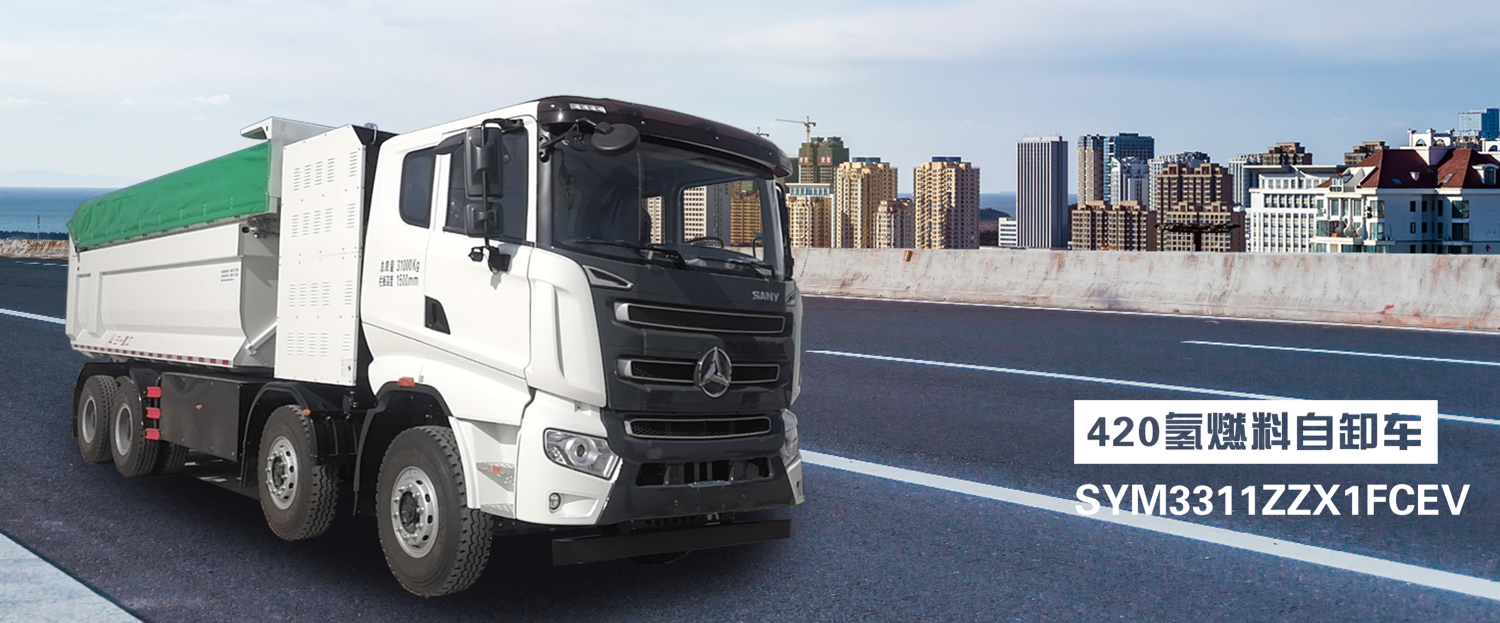
\includegraphics[scale=0.3]{p7.png}
\caption{三一重工氢能源重卡}
\end{figure}

\section{可能的数字化方向}
\subsection{防爆保障}
安全一直是氢能源车辆的短板,氢气比其他燃料或气体泄漏速率更快:在层流状态下,氢气的泄漏速率约为甲烷的 1.26 倍,而在高压下,氢气往往处于湍流状态,此时它的泄漏速率更快,约为甲烷的 2.83 倍。另外,氢气极易扩散,其在薄膜中的扩散速度约为甲烷的 3.8 倍。在非受限空间内,一旦发生意外泄漏,由于氢气密度比空气低,会迅速上浮并向四周扩散。而在受限空间,泄漏的氢气易于在局部聚积,由于其高扩散性,能够快速形成危险的可燃性混合物。

此外,氢气还会引发特有的氢脆破坏。特别是在高压氢气系统中,随着压力增大,高强度钢材长期暴露在氢环境中很容易发生氢脆。有一种解释是,氢气会在钢材表面解离为氢原子并渗入,在外应力作用下,氢聚集在钢内部造成应力集中从而引发局部开裂。

\begin{figure}[htbp]
\centering
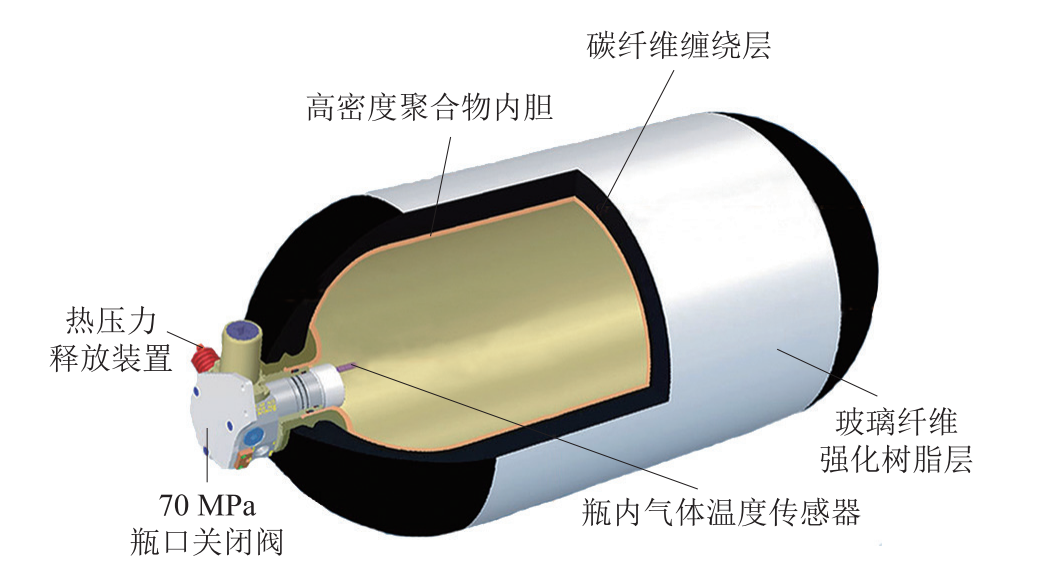
\includegraphics[scale=0.45]{p8.png}
\caption{IV 型轻质高压气态储氢瓶模型图}
\end{figure}

目前,氢能源重卡主要的储氢技术为高压气态储氢。高压气态储氢是一种最常见、应用最广泛的储氢方式,其利用气瓶作为储存容器,通过高压压缩方式储存气态氢。目前,高压气态储氢容器主要分为纯钢制金属瓶(I 型)、钢制内胆纤维缠绕瓶(II 型)、铝内胆纤维缠绕瓶(III 型)及塑料内胆纤维缠绕瓶(IV 型)。

因此,我们可以在储氢容器内外装入精密的化学传感器,在容器内部加入精密的压力传感器,并进行联网,对泄漏和氢脆现象进行及时有效的预警,减少氢气爆炸的风险。

\subsection{电池状态监测}

燃料电池是氢能源卡车的心脏,其运行的情况直接关系到卡车的性能和寿命。若使用各类传感器对电池进行综合联网检测,可以做到遇到问题及时检修,与控制系统配合增强卡车性能。

例如,质子交换膜燃料电池的毒化问题。铂催化剂极富活性, 因而提供了优异的性能。 该催化剂高度活性的制约在于其对一氧化碳和硫的生成物与氧相比有较高的亲合力。 毒化效应强烈地约束了催化剂, 并阻碍了扩展到其中的氢或氧。但是,我们可以通过数字化控制,向阳极气流中增加一氧化碳,由一氧化碳引起的毒化是可逆的,从而解决毒化问题。

再例如,PEMFC 中,影响电堆运行状态的参数有很多,如氢气流量、温度及湿度,空气流量、温度及湿度,冷却水流量等外部参数和电堆内部温度等其他物理参数,系统的各项参数均对 PEMFC 的运行状态和性能有重要影响,可从中筛选并作为故障诊断的特征参数。图9是一个稳压联合检测系统示意图。

\begin{figure}[htbp]
\centering
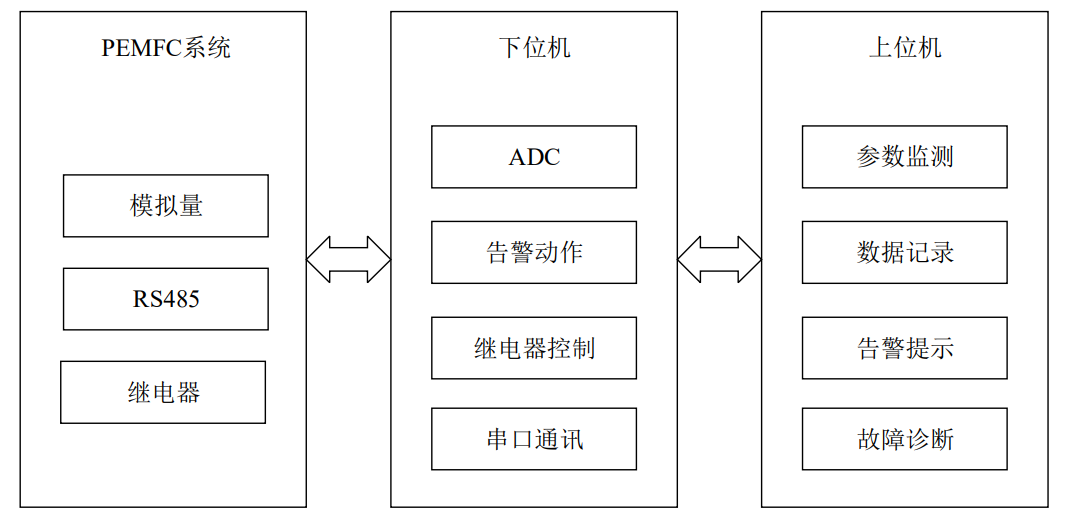
\includegraphics[scale=0.45]{p9.png}
\caption{安全监测系统总体结构}
\end{figure}



\section{参考资料}
为了阅读者直接参考的方便,本笔记的参考资料并不是使用GB/T 7714-2015 格式引文的标准呈现的。

本笔记关于电动汽车和燃料电池系统的参考来自于机械工业出版社的《现代电动汽车、混合动力电动汽车和燃料电池车——基本原理、理论》,电子书网址是\url{https://annas-archive.org/md5/efe11404804193fde58bc8cf69c3c935}。

对氢能源重卡市场情况及其优势的介绍,来自这篇文章,网址为\url{https://www.36kr.com/p/1607306213641345}。

关于近期中国氢能重卡行业的介绍,主要参考了《2023年中国氢能重卡行业词条报告》,网址为\url{https://pdf.dfcfw.com/pdf/H3_AP202305191586976547_1.pdf?1684527706000.pdf}。一些主要参与公司网站如下:亿华通\url{http://www.sinohytec.com/}、三一重工氢能源\url{https://www.sanygroup.com/product/726.html}。

关于氢气和车载储氢技术的安全问题,主要参考了北京市氢燃料电池发动机工程技术研究中心张志芸《车载储氢技术研究现状及发展方向》,知网网址\url{https://kns.cnki.net/kcms2/article/abstract?v=3uoqIhG8C44YLTlOAiTRKibYlV5Vjs7i0-kJR0HYBJ80QN9L51zrP2nVa5E9JgOzKm16o-e2lDC03wgbEW-mZMBITnpEkku2&uniplatform=NZKPT&src=copy},以及华东理工大学沈晓波《高压氢气泄漏相关安全问题研究与进展》,知网网址\url{https://kns.cnki.net/kcms2/article/abstract?v=3uoqIhG8C44YLTlOAiTRKibYlV5Vjs7iy_Rpms2pqwbFRRUtoUImHX8YO2gOcNhjoNSkHQO3t312_FEK6MU2gn4jYxKaTRuE&uniplatform=NZKPT&src=copy}。

关于温压联合检测系统,主要参考了太原理工大学刘奥《氢燃料电池安全监测系统设计与故障诊断方法研究》,知网网址为:\url{https://kns.cnki.net/kcms2/article/abstract?v=3uoqIhG8C475KOm_zrgu4lQARvep2SAkueNJRSNVX-zc5TVHKmDNklY41SpQOgJC9D-shskWKqhjIujOAhpEye97t0S73fbx&uniplatform=NZKPT&src=copy}。

\end{document}